\section{Information extraction}\label{sec:information_extraction}

The information extraction module is responsible for extracting relevant product information from the product pages, such as the name of the product, its price, image, and availability.
Similar to the page classifier module, the information extraction module is also trained using a labelled dataset of HTML pages, which is created using the data annotation application.
The information extraction module is able to accurately extract product information by analyzing the content and structure of the minimized HTML pages.

The information extraction process takes place in three phases.
\begin{enumerate}
    \item \textbf{Training phase:} In this phase, different information extraction models are trained/fine-tuned using the labelled dataset of HTML pages.
    The training phase involves model selection, and model training, fine-tuning, and hyperparameter tuning.
    \item \textbf{Model evaluation and selection:} In this phase, the trained models are evaluated using a separate validation dataset, and the best performing model is selected for deployment.
    Other factors such as training/inference speed and cost are also considered when selecting the best model.
    \item \textbf{Inference phase:} In this phase, the trained information extraction model is used to extract relevant product information from newly crawled product pages.
    \item \textbf{Price history tracking}: In this phase, whenever a product's information is extracted, its price is recorded with the timestamp so that its historical price can be tracked.
\end{enumerate}

\subsection{Training phase}\label{subsec:information_extraction_training_phase}

Since the dataset is once again unstructured, consisting of HTML pages with varying content and structure, a deep learning approach is used for the information extraction task as well.
For the information extraction task, three different techniques were trained and evaluated.
\begin{itemize}
    \item \textbf{MarkupLM for token classification:} This approach involves using a pre-trained MarkupLM model, which is specifically designed for processing HTML documents, to classify the tokens in the HTML content into different product information categories (e.g., name, price, image, availability).
    \item \textbf{Multi-modal approach with LayoutLMv3:} This approach involves using a multi-modal model that combines textual and visual information from the HTML pages to extract product information.
    \item \textbf{LLM based approach:} This approach involves using a large language model (LLM) to extract product information from the HTML pages by leveraging its natural language understanding capabilities.
\end{itemize}

\subsubsection{Using MarkupLM for token classification}
MarkupLM is a pre-trained model that is specifically designed for processing HTML/XML documents, and it has been shown to perform well on various document understanding tasks.
With this approach, the task essentially becomes a token classification problem, where each token in the HTML content is classified into one of the product information categories.
\begin{itemize}
    \item \textbf{\texttt{TITLE-TOKEN}:} This category represents the tokens that belong to the product title.
    \item \textbf{\texttt{PRICE-TOKEN}:} This category represents the tokens that belong to the product price.
    \item \textbf{\texttt{IMAGE-TOKEN}:} This category represents the tokens that belong to the product image URL.
    \item \textbf{\texttt{OUT-OF-STOCK-TOKEN}:} This category represents the tokens that indicate that the product is out of stock.
    \item \textbf{\texttt{NULL-TOKEN}:} This category represents the tokens that do not belong to any of the above categories.
\end{itemize}

The \textttt{OUT-OF-STOCK-TOKEN} was selected as most sites do not explicitly mention the availability of a product, but rather indicate that a product is out of stock when it is unavailable for purchase.
This token is identified by the presence of certain keywords in the HTML content, such as "out of stock", "unavailable", "sold out", etc.

The implementation of this approach first involved the conversion of the labelled dataset into a format suitable for token classification, where each token in the HTML content is assigned a label corresponding to its category.
This was done via\. a custom pre-processing script that tokenizes the HTML content of a minimized page and assigns labels to each token based on the annotated product information in the labelled dataset.
For example, for the product title, there would be two types of tokens named \texttt{B-TITLE} and \texttt{I-TITLE}, where \texttt{B-TITLE} represents the first token of the product title and \texttt{I-TITLE} represents the subsequent tokens of the product title.
Figure~\ref{fig:information_extraction_markuplm_training} illustrates how the pre-processing script would assign labels to the tokens in the HTML content of a minimized page based on the annotated product information in the labelled dataset.

\begin{figure}[h]
    \centering
    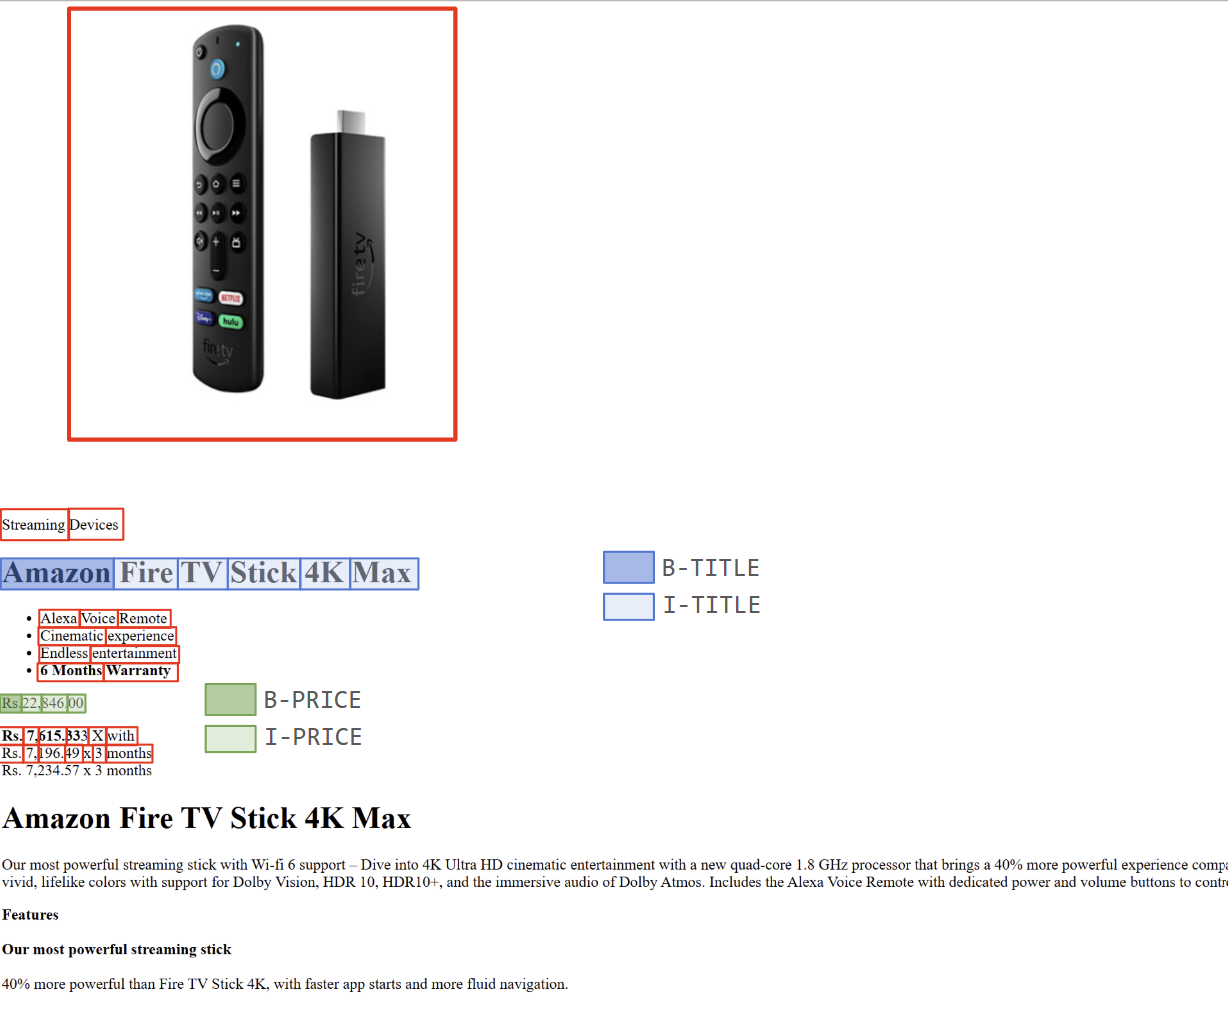
\includegraphics[width=0.6\textwidth]{images/page-tokenization}
    \caption{Example of how a product page is tokenized with the \texttt{B-} and \texttt{I-} classes}
    \label{fig:information_extraction_markuplm_training}
\end{figure}

With this tokenized dataset, the MarkupLM model was fine-tuned for the token classification task using the labelled dataset of HTML pages.
Similar to the page classification model, the hyperparameters of the MarkupLM model were tuned using a grid search approach available in AWS SageMaker.
Figure ~\ref{fig:markuplm_extraction_model_training} illustrates how the MarkupLM model was fine-tuned for the token classification task.

\begin{figure}[h]
    \centering
    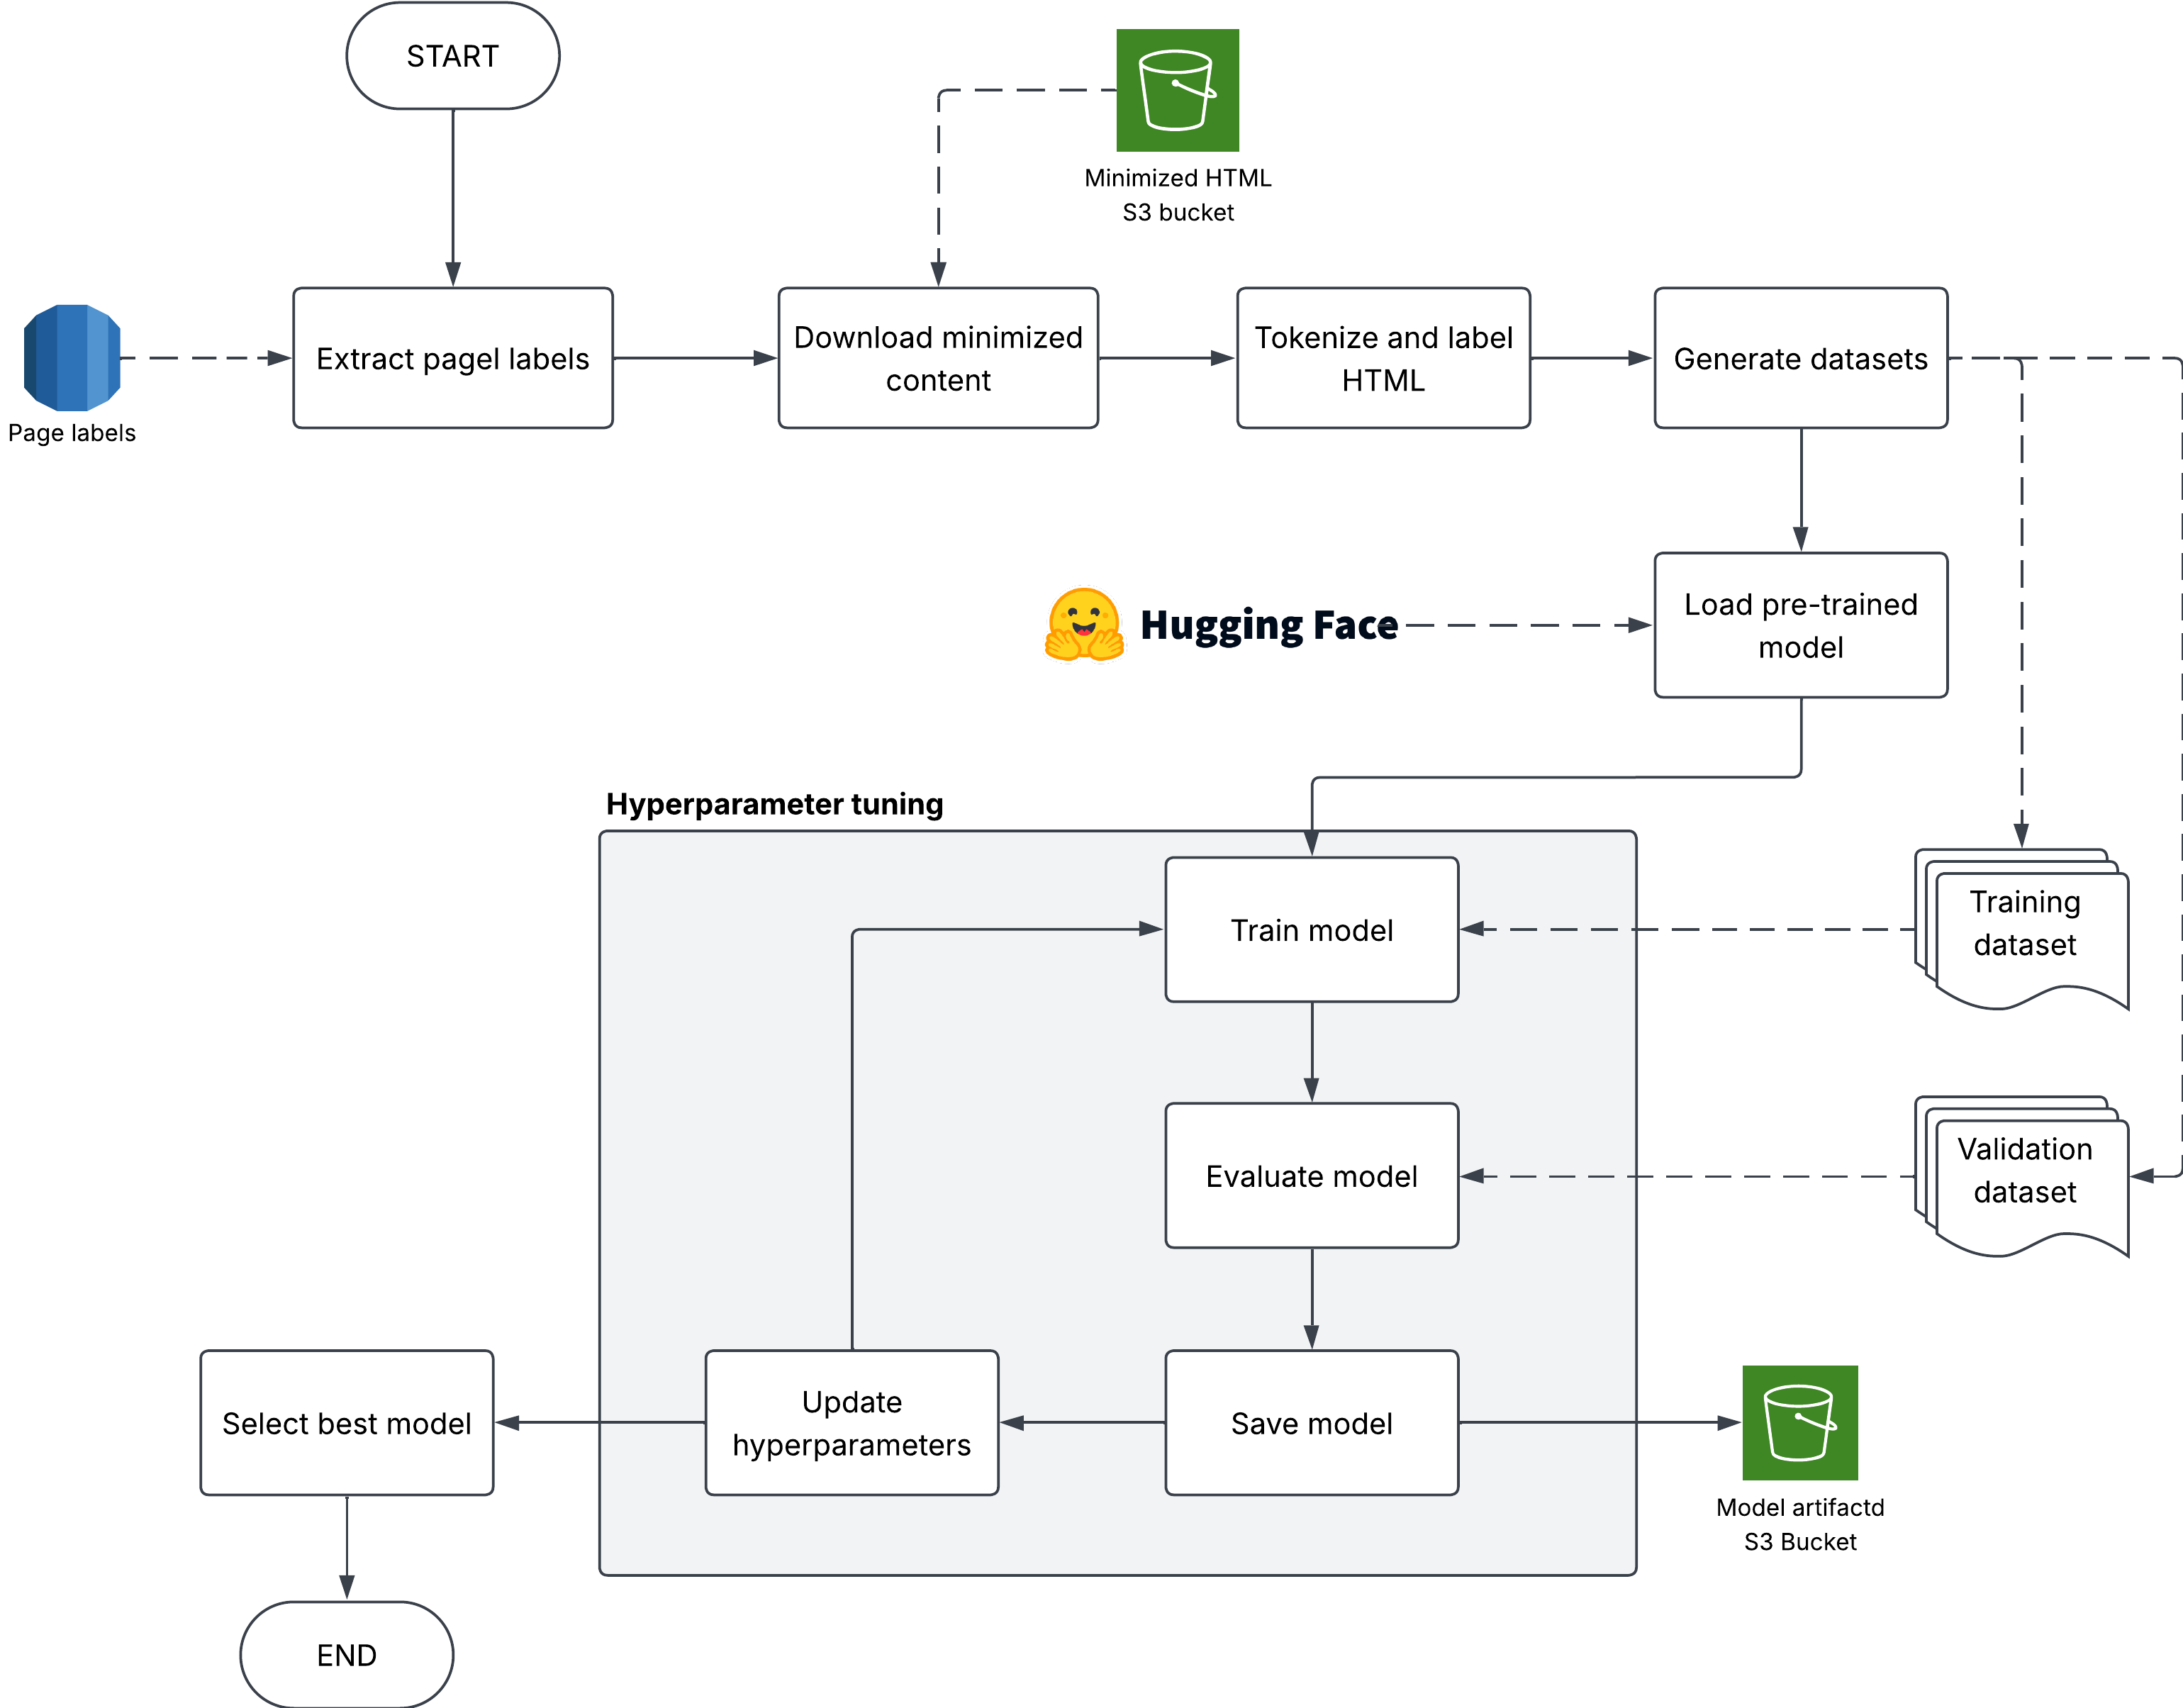
\includegraphics[width=1\textwidth]{images/markuplm_extraction_model_training}
    \caption{Overview of the information extraction model training phase.}
    \label{fig:markuplm_extraction_model_training}
\end{figure}

During the training phase, it was observed that the MarkupLM model did not perform well at classifying the tokens correctly.
This waa primarily due to the high cardinality of the token classes, with two classes for each product information category (e.g., \texttt{B-TITLE} and \texttt{I-TITLE} for the product title), which made it difficult for the model to learn the correct token classifications.
The solution was to drop the~\texttt{I-} classes and keep only the \texttt{B-} classes for each product information category, which reduced the number of token classes and improved the model's performance.
Figure~\ref{fig:information_extraction_model_training} illustrates how the pre-processing script would assign labels to the tokens in the HTML content of a minimized page based on the annotated product information in the labelled dataset, with only the \texttt{B-} classes.

\begin{figure}[h]
    \centering
    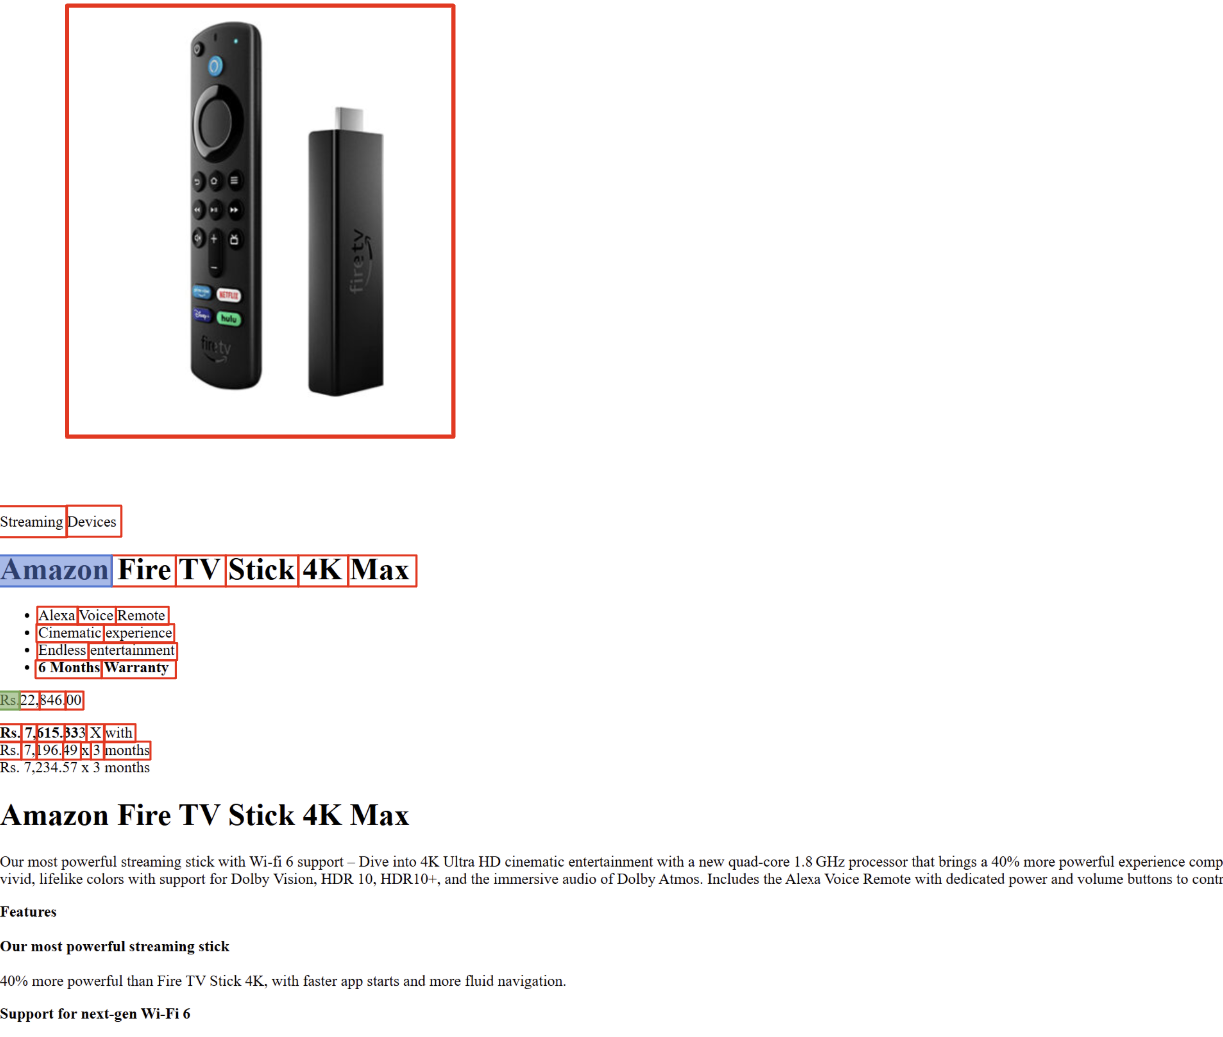
\includegraphics[width=0.6\textwidth]{images/token_classification_2}
    \caption{Example of how a product page is tokenized with only the \texttt{B-} classes}
    \label{fig:information_extraction_model_training}
\end{figure}

With this tokenized dataset, the performance of the model improved significantly, and the model was able to accurately classify the tokens in the HTML content into the correct product information categories.

\subsubsection{Multi-modal approach with LayoutLMv3}

This approach involved using a multi-modal model that combines textual and visual information from the HTML pages to extract product information.
The LayoutLMv3 model was used for this purpose, which is a pre-trained model that is specifically designed for document understanding tasks that involve both textual and visual information.

Similar to the MarkupLM approach, there involved a pre-processing step which combined the HTML content of a page with the labelled product information in the labelled dataset to create a multi-modal dataset suitable for training the LayoutLMv3 model.
\begin{enumerate}
    \item The original HTML content (not minimized) of a product page was converted into an image using a headless browser, which rendered the HTML content and captured a screenshot of the page.
    \item The labelled product information in the labelled dataset was used to create bounding boxes around the relevant product information in the image of the product page.
    The bounding boxes were created using the coordinates of the HTML elements corresponding to the labelled product information.
    \item The bounding boxes were then labelled with the corresponding product information category (e.g., name, price, image, availability) to create a multi-modal dataset suitable for training the LayoutLMv3 model.
\end{enumerate}

Figure~\ref{fig:layoutlmv3_extraction_model_training} illustrates how the pre-processing script would create bounding boxes around the relevant product information in the image of a product page based on the annotated product information in the labelled dataset.

\begin{figure}[h]
    \centering
    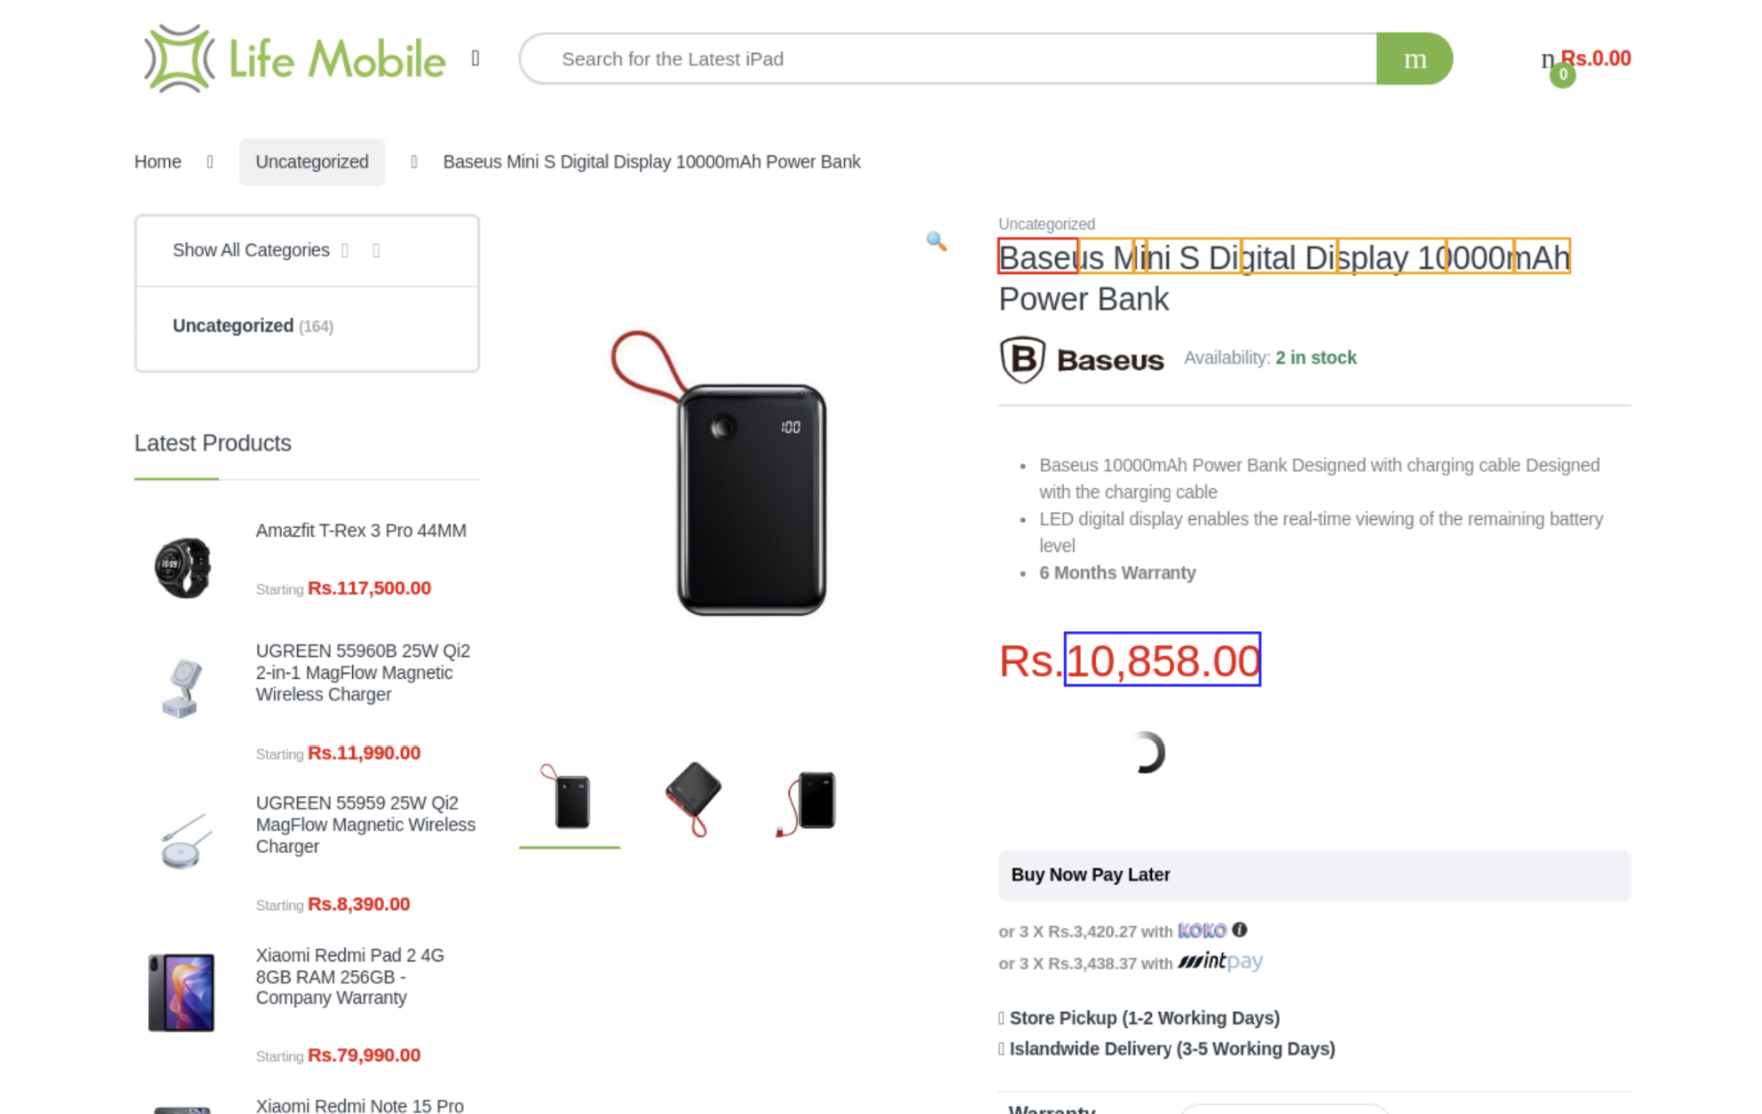
\includegraphics[width=1\textwidth]{images/layoutlm_preprocessing}
    \caption{Example of bounding boxes created around the relevant product information in the image of a product page}
    \label{fig:layoutlmv3_extraction_model_training}
\end{figure}

After this pre-processing stage, the LayoutLMv3 model was fine-tuned for the information extraction task using the labelled dataset of HTML pages, similar to the MarkupLM approach.
The hyperparameters of the LayoutLMv3 model were also tuned using a grid search approach available in AWS SageMaker.

\subsubsection{LLM based approach}

The LLM based approach was comparatively simpler than the other two approaches, as it did not require any pre-processing of the HTML content or the training/fine-tuning of a model.
Instead, the LLM was used to extract product information from the HTML content of a product page by providing it with a prompt that describes the task and the expected output format.
Two LLM models were evaluated for this approach, Google's Gemini 2.5 Flash Lite and Google's Gemini 2.5 Flash.
The LLM was able to accurately extract product information from the HTML content by leveraging its natural language understanding capabilities.

\subsection{Model evaluation and selection}\label{subsec:information_extraction_model_evaluation}
The three approaches were evaluated using a separate validation dataset, and the best performing model was selected for deployment.
For this phase, only the extraction of the product title and price was considered, as the extraction of the product image and availability was not a priority for the proof-of-concept system.

The comparative results are summarized in Table~\ref{tab:information_extraction_results}.

\begin{table}[h]
    \centering
    \small
    \renewcommand{\arraystretch}{1.4}
    \begin{tabularx}{\textwidth}{p{4cm} p{2.1cm} p{2.1cm} X X}
        \toprule
        \textbf{Technique} & \textbf{Title Accuracy} & \textbf{Price Accuracy} & \textbf{Pre-processing time \& cost (for 20,000 pages)} & \textbf{Extraction time \& cost (for 20,000 pages)} \\
        \midrule
        MarkupLM &
        0.951 &
        0.920 &
        \begin{minipage}[t]{\linewidth}\centering 22 mins\\\$0.14\end{minipage} &
        \begin{minipage}[t]{\linewidth}\centering 7 mins\\\$0.18\end{minipage} \\
        \midrule
        Multi-modal &
        0.866* &
        0.785* &
        \begin{minipage}[t]{\linewidth}\centering 121 mins\\\$0.88\end{minipage} &
        \begin{minipage}[t]{\linewidth}\centering 13 mins\\\$0.34\end{minipage} \\
        \midrule
        LLM (Gemini 2.5 Flash Lite) &
        0.935 &
        0.970 &
        \begin{minipage}[t]{\linewidth}\centering 10 mins\\\$0.04\end{minipage} &
        \begin{minipage}[t]{\linewidth}\centering 883 mins**\\\$85.85**\end{minipage} \\
        \midrule
        LLM (Gemini 2.5 Flash) &
        0.975 &
        0.960 &
        \begin{minipage}[t]{\linewidth}\centering 10 mins\\\$0.04\end{minipage} &
        \begin{minipage}[t]{\linewidth}\centering 1,576 mins**\\\$281.68**\end{minipage} \\
        \bottomrule
    \end{tabularx}
    \caption{Comparison of information extraction approaches}
    \label{tab:information_extraction_results}
\end{table}

\noindent All models were trained and then tested against data from websites they had not been exposed to.
\begin{itemize}
    \item[*] The performance of the multi-modal model could be improved with further training and fine-tuning, but not enough to justify the additional cost.
    \item[**] Extraction time and cost for the LLM approaches are estimated based on a sample of 200 pages.
    \item[**] Extraction time for the LLM approaches could be improved through parallelization.
\end{itemize}

Although the LLM based approach achieved the highest accuracy for both title and price extraction, it was not selected for deployment due to its high inference time and cost.
The MarkupLM approach was selected for deployment as it achieved a good balance between accuracy, inference time, and cost, making it suitable for the information extraction task in the proposed system.

\subsection{Inference phase}\label{subsec:information_extraction_inference_phase}
In the inference phase, the trained MarkupLM model is used to extract relevant product information from newly crawled product pages.
The inference process involves the following steps:
\begin{enumerate}
    \item Extract the newly crawled product pages which have not yet been processed by the information extraction model.
    \item For each page, download the minimized HTML content from the S3 bucket.
    \item Pre-process the HTML content to tokenize it and assign labels to each token based on the product information categories.
    \item Feed the tokenized HTML content into the fine-tuned MarkupLM model to classify the tokens into the product information categories.
    \item Post-process the output of the MarkupLM model to extract the relevant product information (e.g., name, price, image, availability) from the classified tokens.
    \item Store the extracted product information in the database, along with the relevant metadata, such as the page URL and the timestamp of the extraction.
\end{enumerate}

The post-processing step intends to solve several problems that arise from the token classification output of the MarkupLM model.
\begin{itemize}
    \item \textbf{Only the beginning of the product information is classified:} Since only the \texttt{B-} classes were used for token classification, the MarkupLM model only classifies the beginning of the product information (e.g., the first token of the product title or price).
    \item \textbf{Cleaning the extracted product information:} The output of the MarkupLM model may contain extraneous tokens that are not part of the actual product information (e.g., HTML tags, special characters, etc.).  These extraneous tokens are removed during the post-processing step to obtain clean product information.
    The post-processing step involves extracting the complete product information by concatenating the subsequent tokens until the end of the parent HTML element is reached.
    \item \textbf{Multiple tokens identified for the same class:} In some cases, the MarkupLM model may classify multiple tokens as belonging to the same product information category (e.g., multiple tokens classified as \texttt{B-TITLE}). This is solved by simply selecting the token with the highest confidence score for each product information category.
    \item \textbf{Identification of pre-sales price and installment prices:} In some cases, the MarkupLM model may classify tokens as belonging to the \texttt{B-PRICE} category, but the identified price may not be the actual selling price of the product.
    For example, some websites may display a pre-sales price or an installment price instead of the actual selling price.
    In such cases, the post-processing step selects the best token through a heuristic approach, which involves selecting the correct token based on its proximity to the selected \texttt{B-TITLE} token and the value of the expanded price (e.g., a price which is ~1/3rd of one of the other visible prices are considered to be installment prices).
    \item \textbf{No tokens identified for a class:} In some cases, the MarkupLM model may not classify any tokens as belonging to a particular product information category (e.g., no tokens classified as \texttt{B-PRICE}).  In cases such as this, it is assumed that the page classification model has misclassified the page as a product page, and the page is ignored.
\end{itemize}

Figure ~\ref{fig:information_extraction_inference_phase} illustrates the post-processing flow and how the correct values for the various product information categories are computed.

\begin{figure}
    \centering
    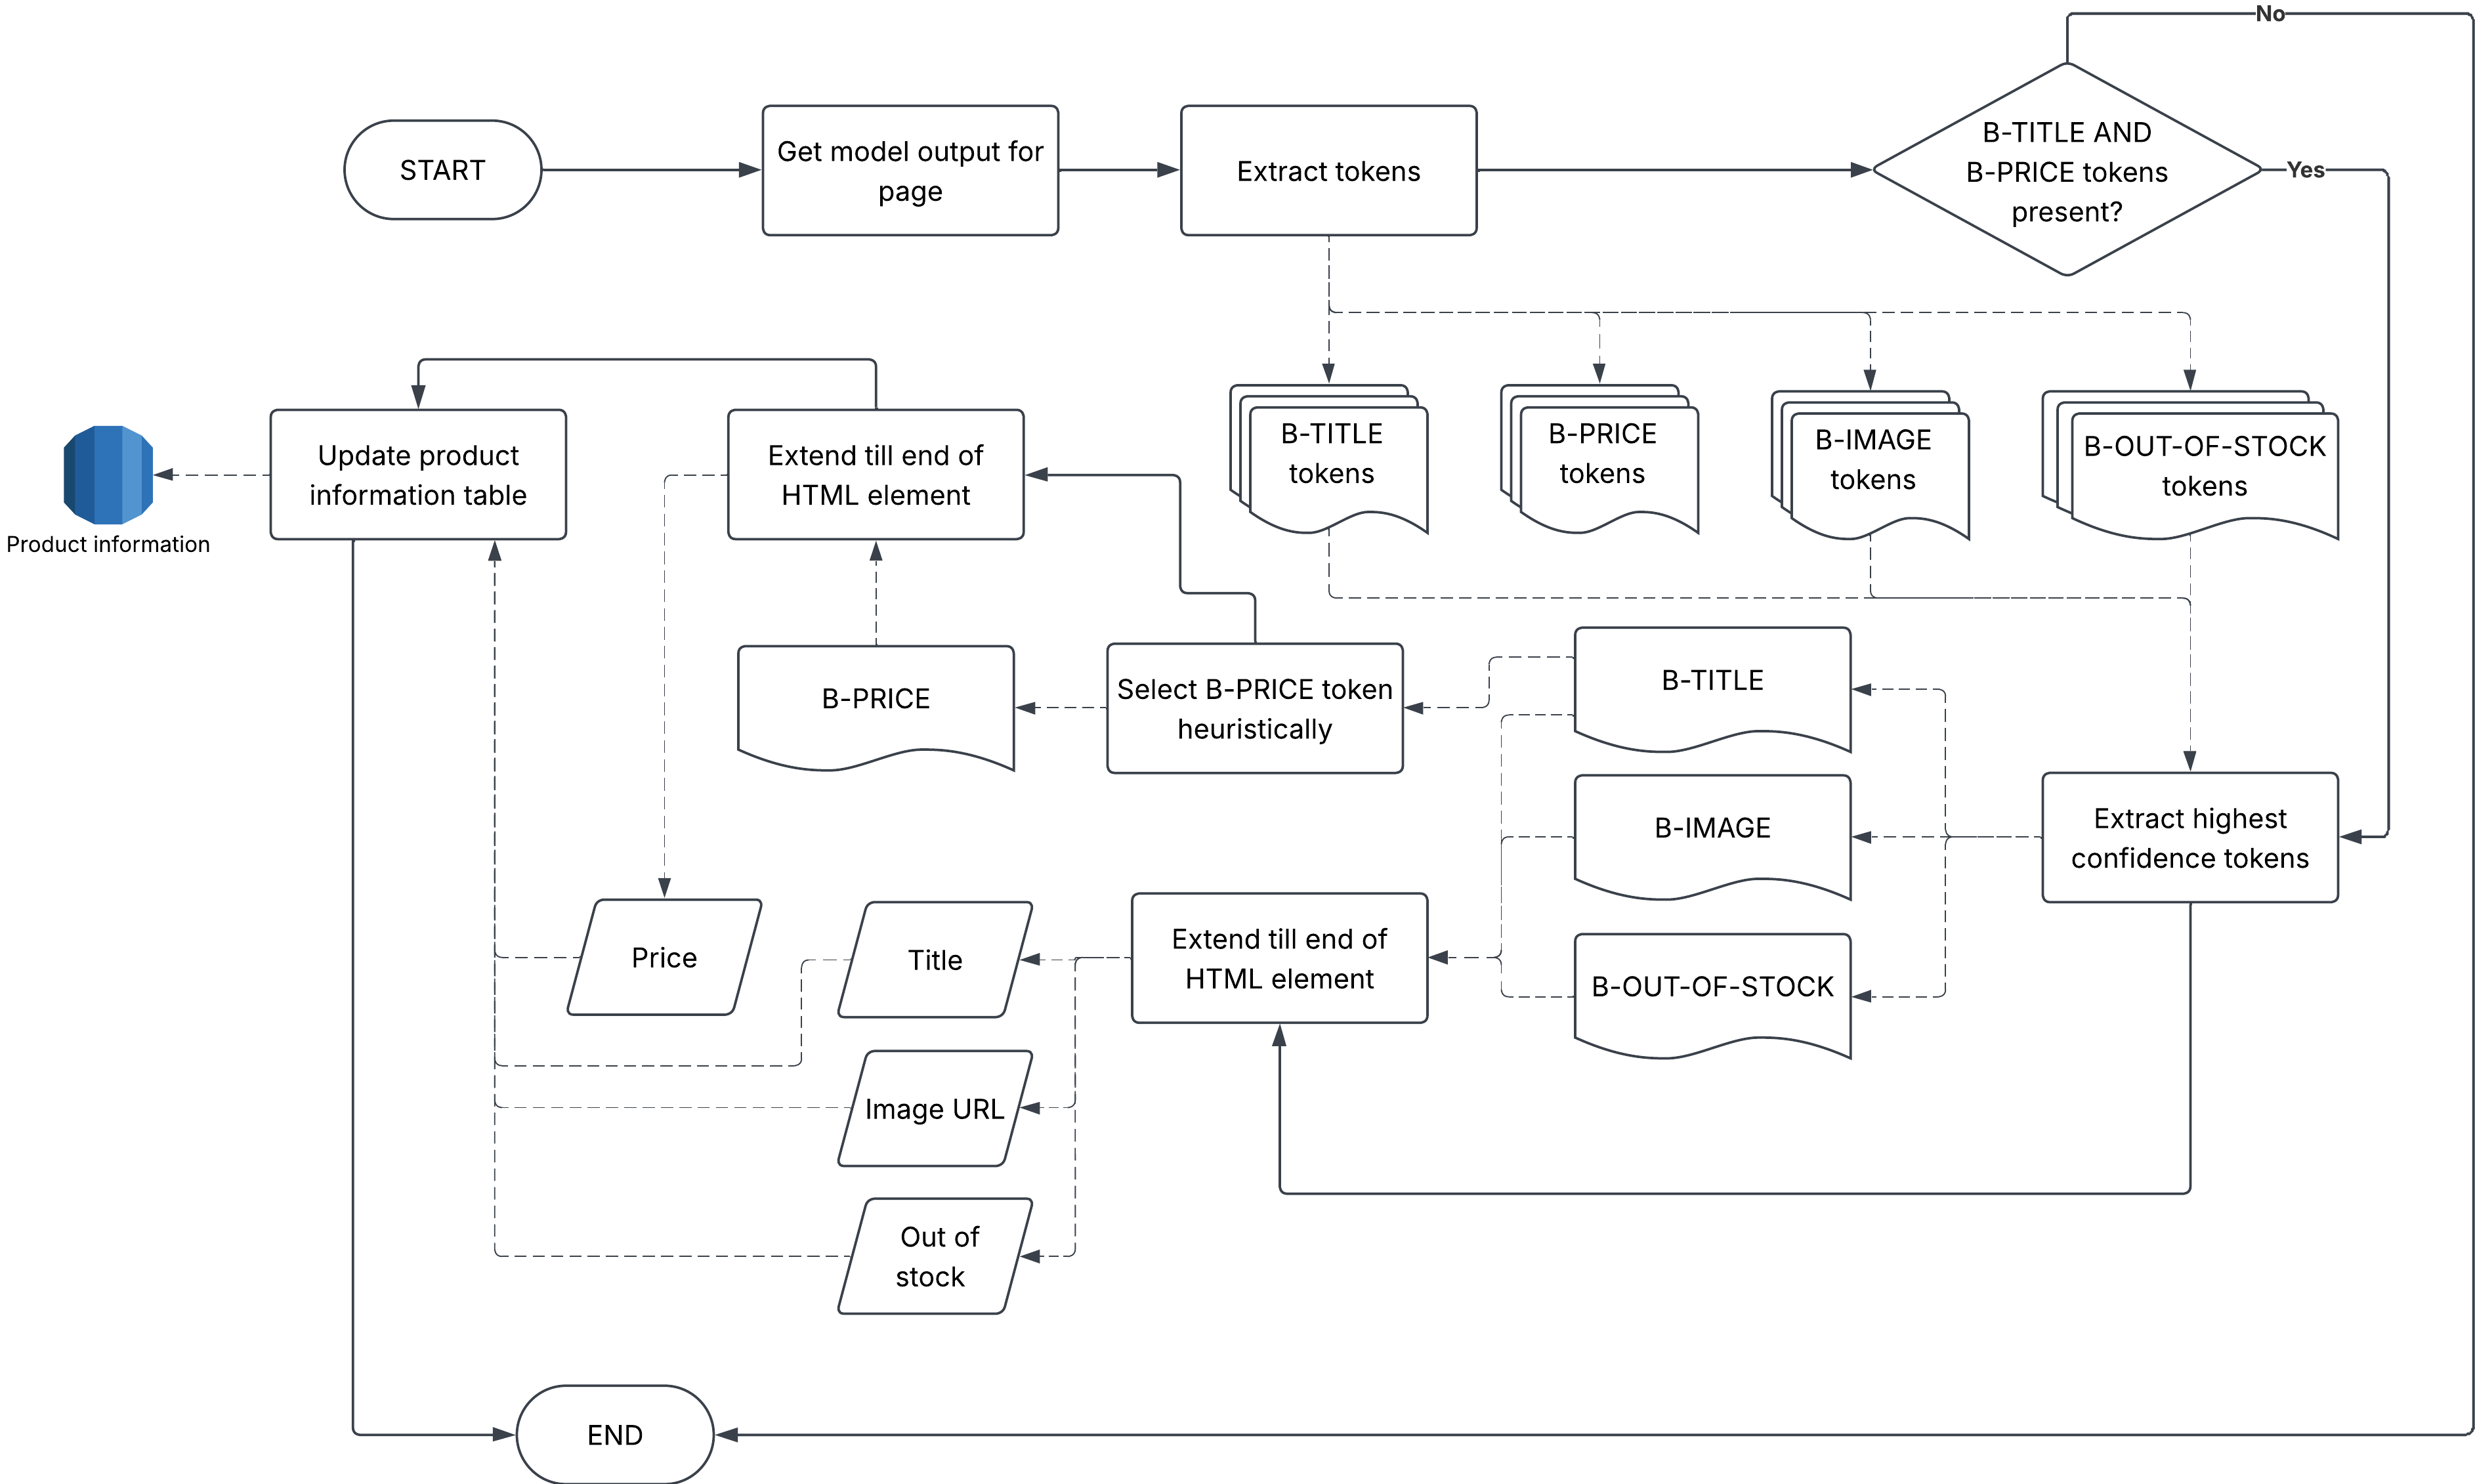
\includegraphics[width=1\textwidth]{images/information_extraction_post_processing}
    \caption{Post-processing flow for information extraction}
    \label{fig:information_extraction_inference_phase}
\end{figure}

\subsection{Price history tracking} \label{subsec:price_history_tracking}
Price history tracking is implemented by using Change Data Capture (CDC) on the product information table.
Whenever a product is updated, its new price is recorded with the last crawled timestamp in the price history table.
This is implemented by using PostgreSQL triggers as shown in Listing~\ref{lst:record_price_change}.
With this approach, a historical record of price snapshots of all products are tracked.

\begin{lstlisting}[language=SQL, caption={Trigger used to record product price changes}, label={lst:record_price_change}, captionpos=b]
CREATE OR REPLACE FUNCTION record_price_change()
    RETURNS TRIGGER AS
$$
BEGIN
    INSERT INTO product_price_history (url, price, recorded_at)
    VALUES (NEW.url, NEW.product_price, NOW());

    RETURN NEW;
END;
$$ LANGUAGE plpgsql;

DROP TRIGGER IF EXISTS trg_record_price_changes ON page_inferred_labels;

CREATE TRIGGER trg_record_price_changes
    AFTER INSERT OR UPDATE
    ON page_inferred_labels
    FOR EACH ROW
EXECUTE FUNCTION record_price_change();
\end{lstlisting}

\subsection{Information extraction module architecture} \label{subsec:information_extraction_module_architecture}

Figure~\ref{fig:information_extraction_module_architecture} illustrates the architecture of the information extraction module, which includes the training phase, inference phase, and price history tracking and how they interact with each other.

\begin{figure}[h]
    \centering
    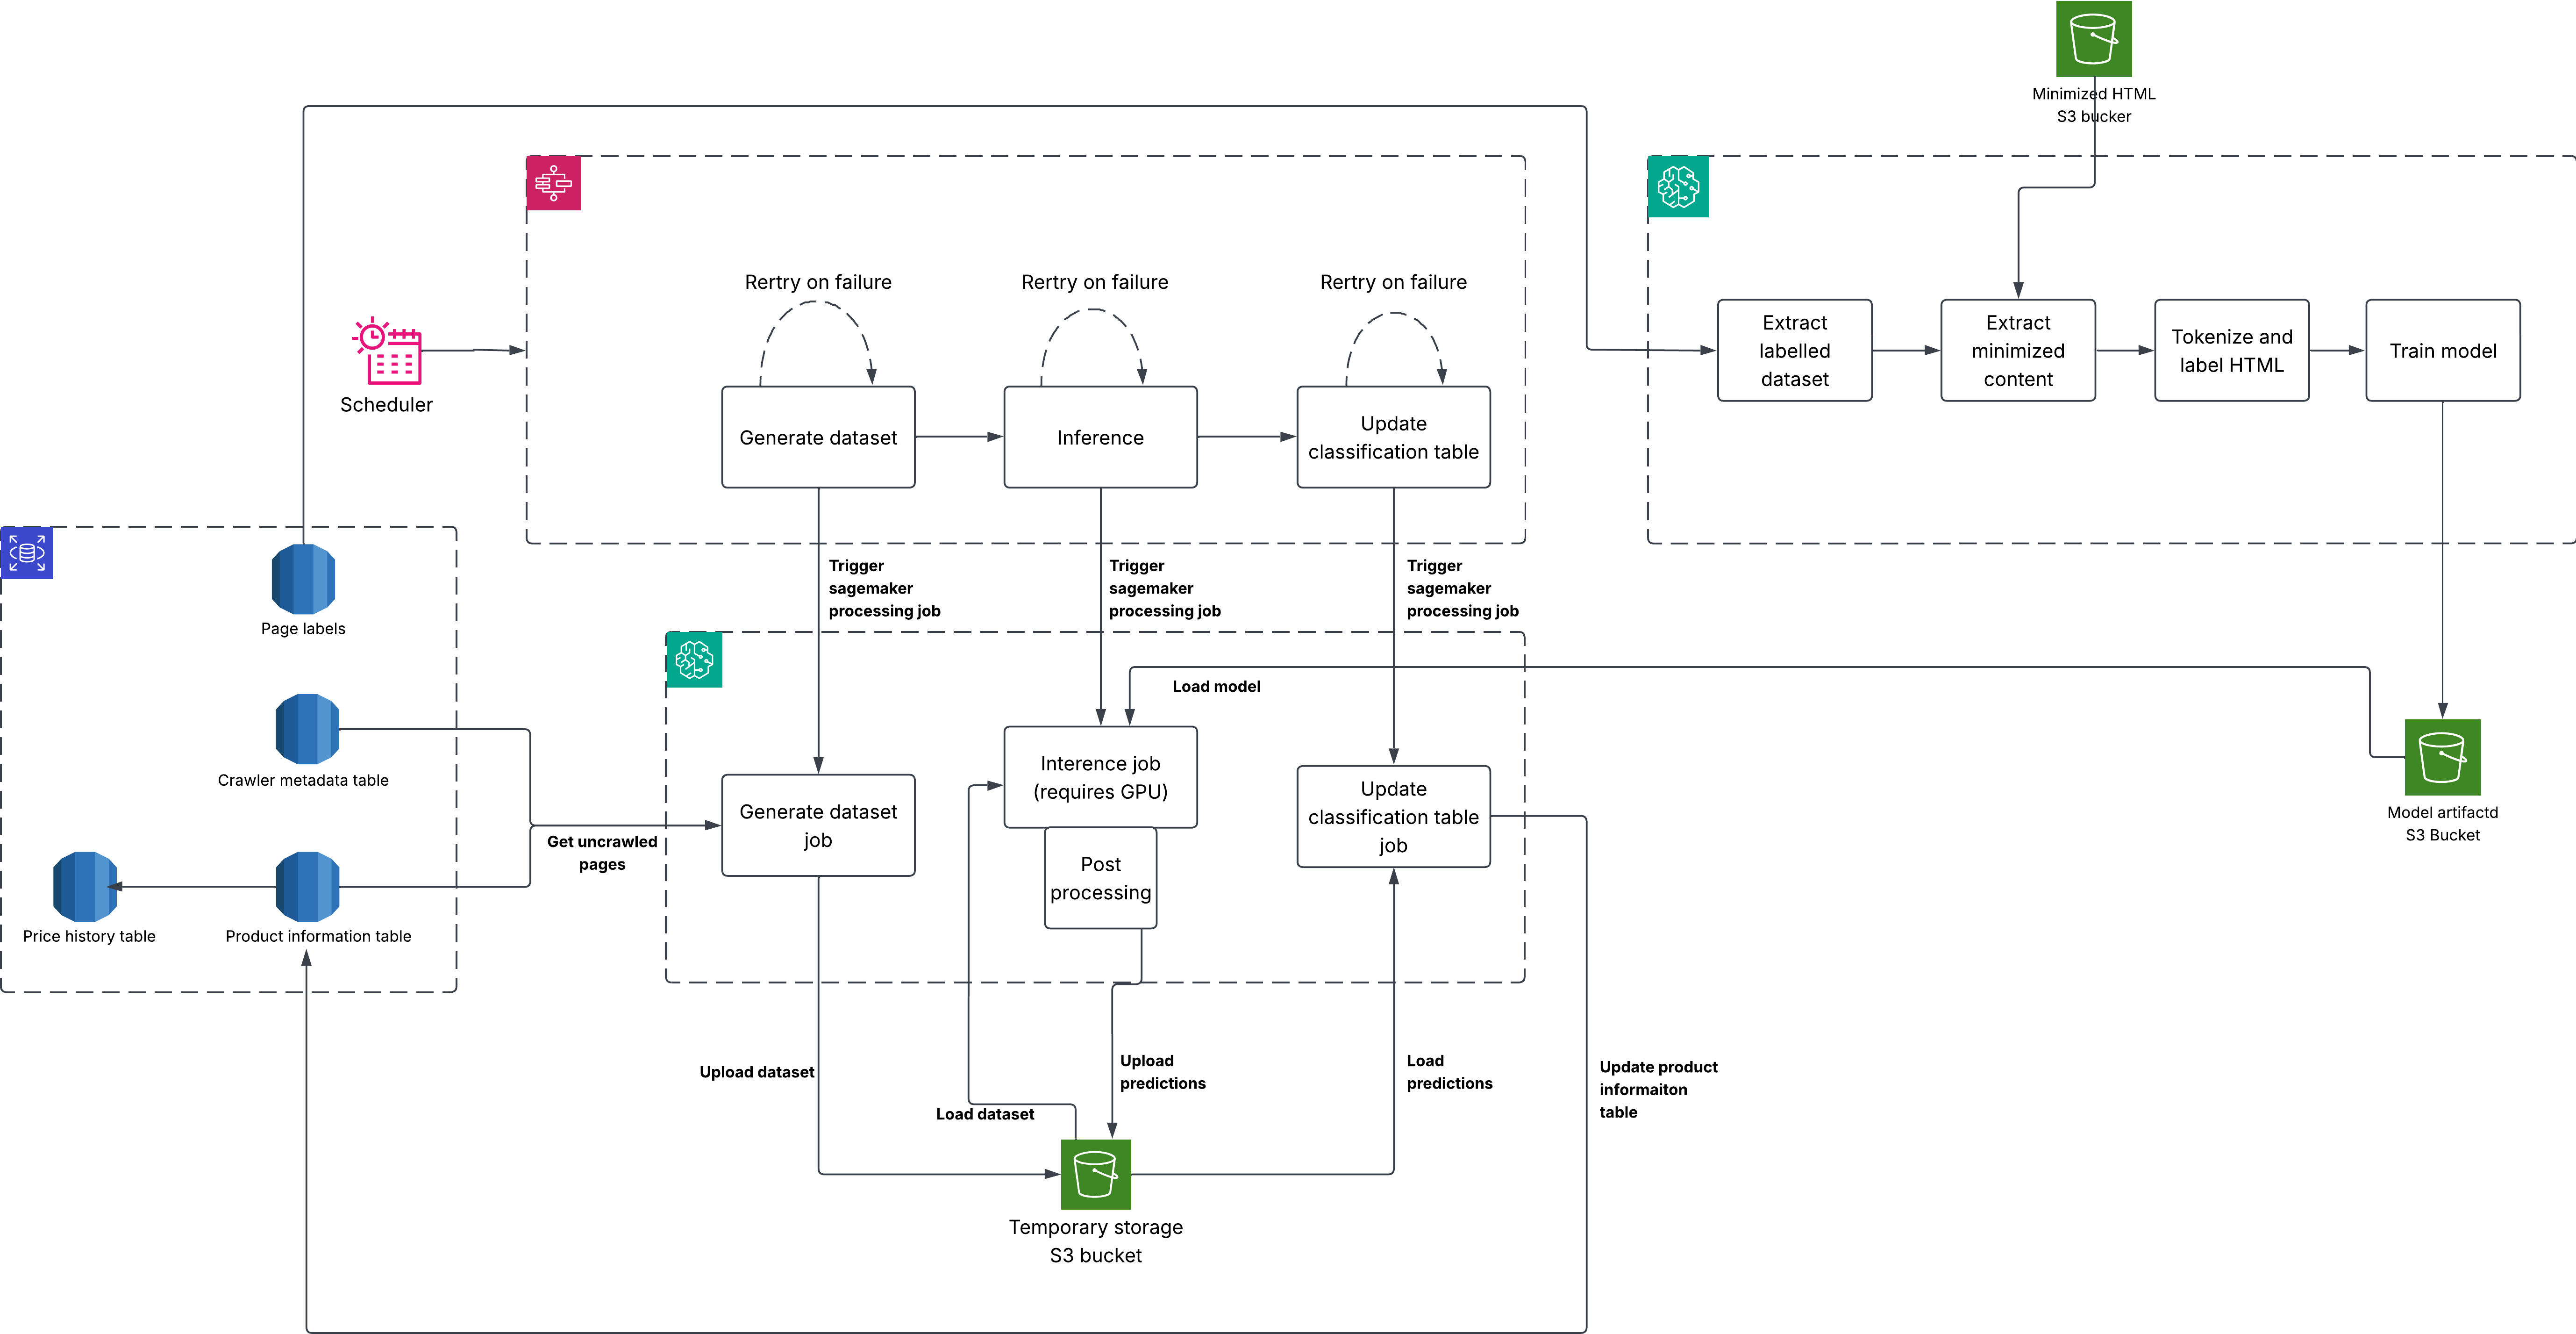
\includegraphics[width=1\textwidth]{images/information_extraction_architecture}
    \caption{Overview of the information extraction module architecture.}
    \label{fig:information_extraction_module_architecture}
\end{figure}